Este capítulo cubre el análisis del sistema de información a desarrollar, haciendo uso del lenguaje de modelado UML.
\section{Casos de uso}
\subsection{Modelo conceptual}
Tras haber identificado los requisitos del sistema, se diseña un diagrama conceptual (Figura ~\ref{fig:modeloER}) que resume las funciones del sistema, así como las relaciones entre los elementos involucrados.

\begin{figure}[H]
    \centering
    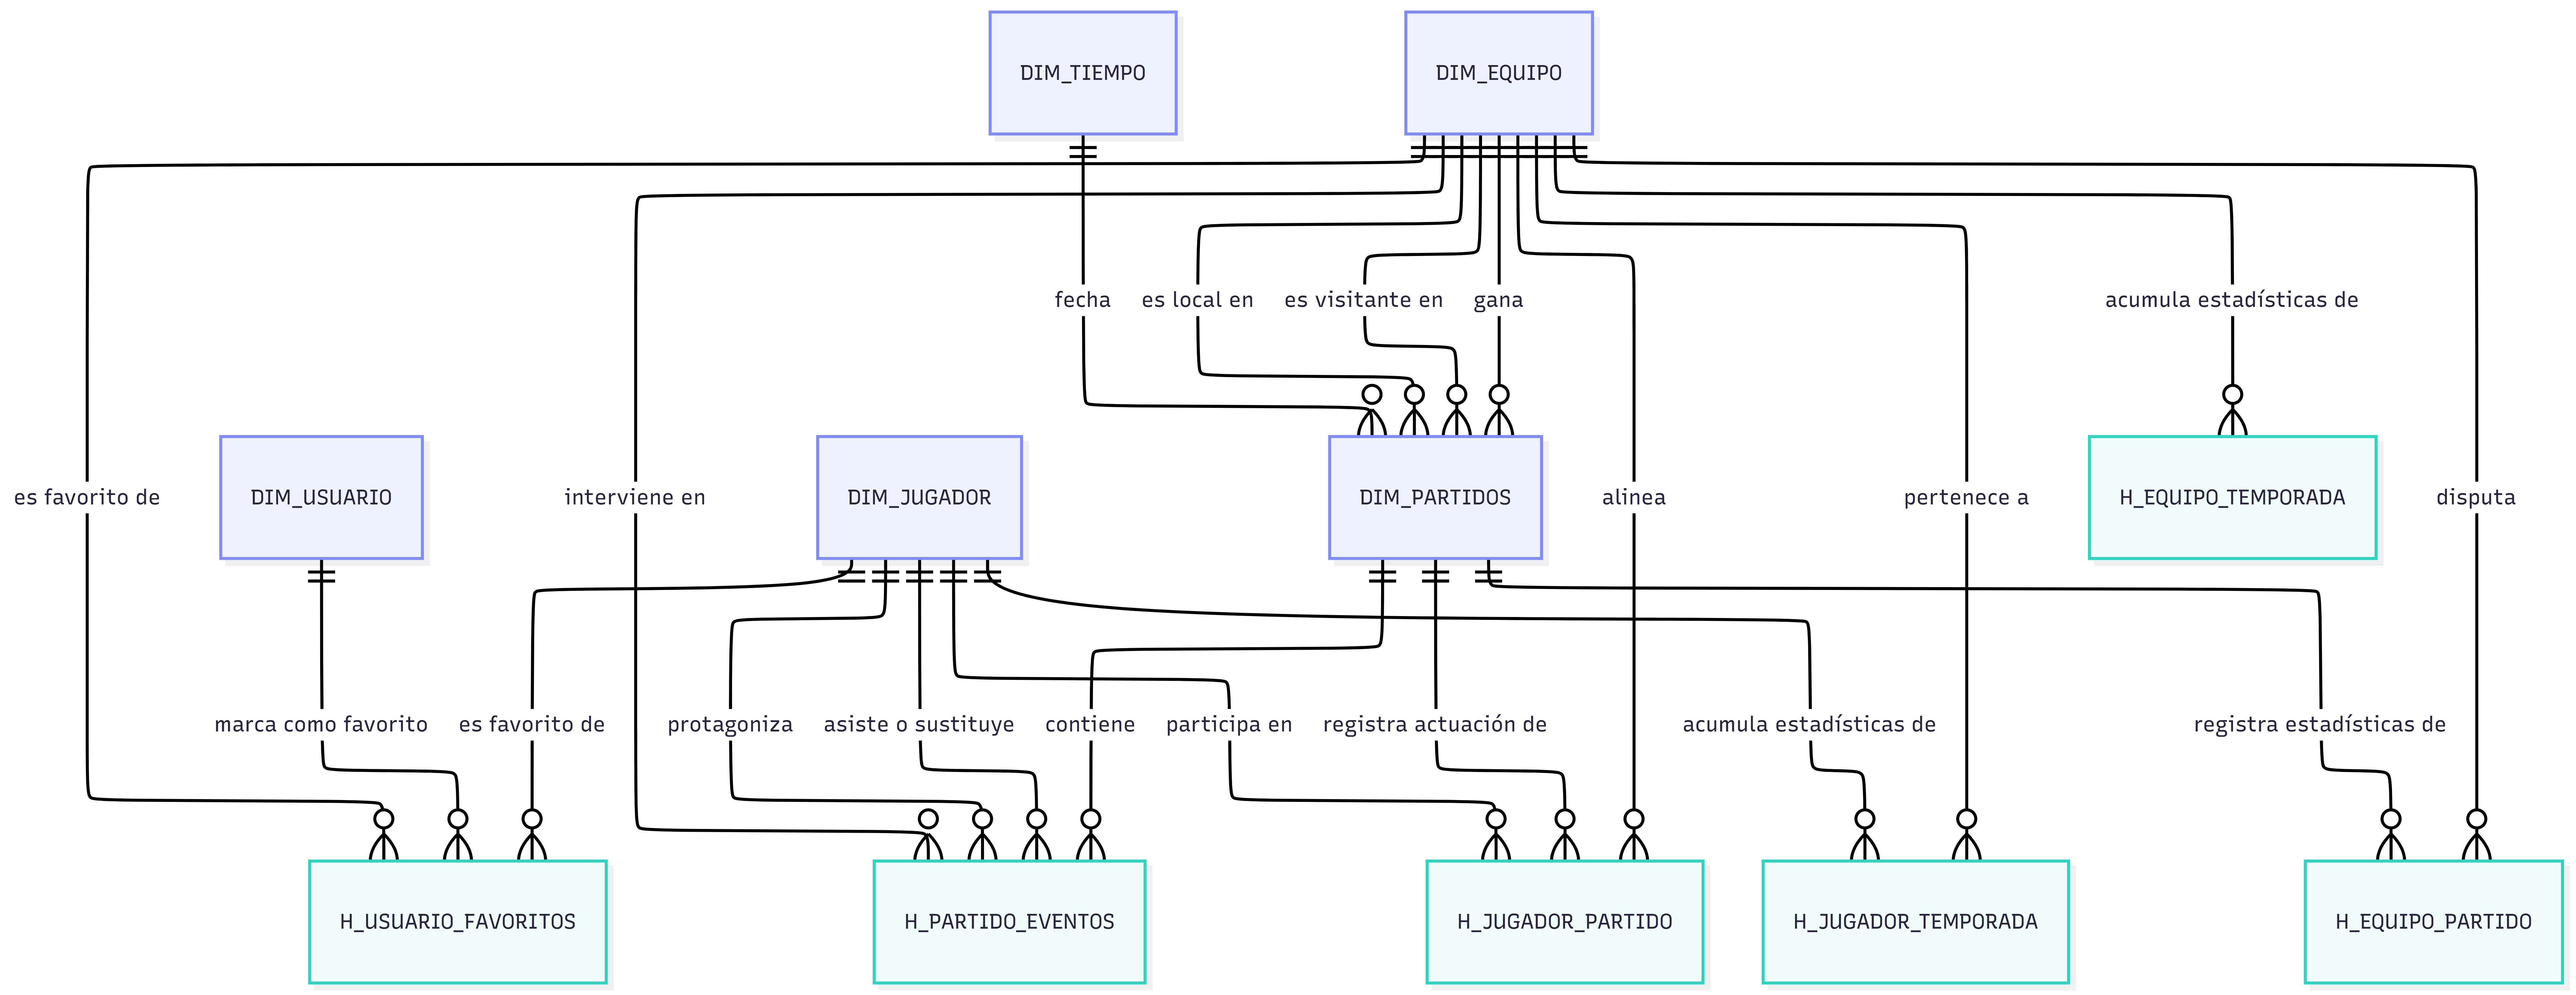
\includegraphics[width=1\linewidth]{figures/modeloER.png}
    \caption{Modelo entidad-relación del DW.}
    \label{fig:modeloER}
\end{figure}

\subsection{Modelo de casos de uso}
\subsubsection{Diagrama de caso de uso}
En este apartado se desarrollarán los casos de uso, los cuales mostrarán las acciones que los actores pueden hacer con el sistema. Específicamente, en este caso, solo tendremos un modelo de caso de uso, que será el de usuario; lo podemos ver en el diagrama de la Figura ~\ref{fig:caso de uso}, creado con la herramienta PlantUML \cite{plantuml}.
\begin{figure}[H]
    \centering
    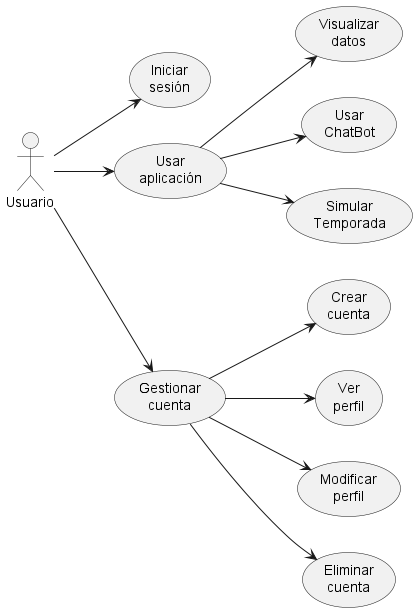
\includegraphics[width=0.6\linewidth]{figures/caso_de_uso.png}
    \caption{Modelo caso de uso: Usuario.}
    \label{fig:caso de uso}
\end{figure}

\subsubsection{Especificación de los casos de uso}

En este apartado se describen los principales casos de uso de la
aplicación. Para cada uno se indican los actores involucrados, las
precondiciones, el flujo principal, los posibles flujos alternativos
y las postcondiciones.

% ----------------------------------------------------------
\subsubsection{CU-01: Crear cuenta}

\noindent \textbf{Actor principal:} Usuario no registrado.

\noindent \textbf{Objetivo:} Crear una cuenta que permita al usuario acceder a las funcionalidades personalizadas de la aplicación.

\noindent \textbf{Precondiciones:} El usuario no ha iniciado sesión y dispone de una dirección de correo electrónico que no está registrada en el sistema.

\noindent \textbf{Disparador:} El usuario selecciona la opción \textit{Regístrate aquí}.

\noindent \textbf{Flujo principal:}
\begin{enumerate}
    \item El sistema muestra el formulario de registro.
    \item El usuario introduce su nombre de usuario, correo electrónico y contraseña.
    \item El usuario confirma la contraseña.
    \item El usuario envía el formulario.
    \item El sistema comprueba que los datos introducidos son válidos.
    \item El sistema verifica que el correo electrónico no está registrado.
    \item El sistema crea la cuenta.
    \item El sistema informa al usuario de que el registro se ha completado correctamente.
\end{enumerate}

\noindent \textbf{Flujos alternativos y excepciones:}
\begin{itemize}
    \item Si algún campo obligatorio está vacío, el sistema solicita que sea completado.
    \item Si el correo electrónico no tiene un formato válido, el sistema muestra un mensaje de error.
    \item Si el correo ya está registrado, el sistema informa al usuario y no crea la cuenta.
    \item Si las contraseñas no coinciden, el sistema solicita que se introduzcan de nuevo.
    \item Si la contraseña no cumple los requisitos de seguridad, el sistema informa de los requisitos necesarios.
\end{itemize}

\noindent \textbf{Postcondiciones:} La cuenta queda registrada y el usuario puede iniciar sesión.

\subsubsection{CU-02: Iniciar sesión}

\noindent \textbf{Actor principal:} Usuario registrado.

\noindent \textbf{Objetivo:} Autenticar al usuario para permitirle acceder a las funcionalidades restringidas de la aplicación.

\noindent \textbf{Precondiciones:} El usuario dispone de una cuenta registrada y no ha iniciado sesión.

\noindent \textbf{Disparador:} El usuario abre la aplicación.

\noindent \textbf{Flujo principal:}
\begin{enumerate}
    \item El sistema muestra el formulario de inicio de sesión.
    \item El usuario introduce su correo electrónico y contraseña.
    \item El usuario envía el formulario.
    \item El sistema valida las credenciales.
    \item El sistema inicia la sesión del usuario.
    \item El sistema redirige al usuario a la pantalla principal.
\end{enumerate}

\noindent \textbf{Flujos alternativos y excepciones:}
\begin{itemize}
    \item Si algún campo está vacío, el sistema solicita que sea completado.
    \item Si las credenciales son incorrectas, el sistema muestra un mensaje de error.
    \item Si la cuenta no existe, el sistema informa al usuario y ofrece la posibilidad de registrarse.
    \item Si ocurre un error de conexión, el sistema informa de que no ha sido posible iniciar sesión.
\end{itemize}

\noindent \textbf{Postcondiciones:} La sesión queda iniciada y el usuario puede acceder a las funcionalidades asociadas a su cuenta.

\subsubsection{CU-03: Cerrar sesión}

\noindent \textbf{Actor principal:} Usuario autenticado.

\noindent \textbf{Objetivo:} Finalizar de forma segura la sesión activa del usuario.

\noindent \textbf{Precondiciones:} El usuario ha iniciado sesión previamente.

\noindent \textbf{Disparador:} El usuario selecciona la opción \textit{Cerrar sesión}.

\noindent \textbf{Flujo principal:}
\begin{enumerate}
    \item El usuario abre el menú de su cuenta.
    \item El usuario selecciona la opción \textit{Cerrar sesión}.
    \item El sistema invalida la sesión activa.
    \item El sistema redirige al usuario a la pantalla principal o de inicio de sesión.
\end{enumerate}

\noindent \textbf{Flujos alternativos y excepciones:}
\begin{itemize}
    \item Si la sesión ya ha expirado, el sistema redirige directamente al usuario a la pantalla de inicio de sesión.
    \item Si se produce un error, el sistema elimina localmente los datos de autenticación e informa al usuario.
\end{itemize}

\noindent \textbf{Postcondiciones:} La sesión queda finalizada y las funcionalidades restringidas dejan de estar disponibles.

\subsubsection{CU-04: Visualizar datos de LaLiga}

\noindent \textbf{Actor principal:} Usuario.

\noindent \textbf{Objetivo:} Consultar la información disponible sobre LaLiga, como clasificaciones, equipos, jugadores, partidos o estadísticas.

\noindent \textbf{Precondiciones:} La aplicación está disponible y existen datos almacenados o accesibles desde la fuente de información utilizada.

\noindent \textbf{Disparador:} El usuario accede a la sección de consulta de datos.

\noindent \textbf{Flujo principal:}
\begin{enumerate}
    \item El sistema muestra las categorías de datos disponibles.
    \item El usuario selecciona una categoría.
    \item El sistema obtiene los datos correspondientes.
    \item El sistema presenta la información de forma ordenada.
    \item El usuario puede seleccionar un elemento para consultar sus detalles.
    \item El sistema muestra la información detallada del elemento seleccionado.
\end{enumerate}

\noindent \textbf{Flujos alternativos y excepciones:}
\begin{itemize}
    \item Si no existen datos para la categoría seleccionada, el sistema informa al usuario.
    \item Si la fuente externa de datos no está disponible, el sistema muestra un mensaje de error.
    \item Si el usuario realiza una búsqueda sin resultados, el sistema informa de que no se encontraron coincidencias.
    \item Si existen filtros, el usuario puede aplicarlos y el sistema actualiza la información mostrada.
\end{itemize}

\noindent \textbf{Postcondiciones:} Los datos seleccionados quedan mostrados sin modificar la información almacenada por el sistema.

\subsubsection{CU-05: Consultar al chatbot}

\noindent \textbf{Actor principal:} Usuario.

\noindent \textbf{Objetivo:} Realizar preguntas en lenguaje natural y obtener información relacionada con LaLiga.

\noindent \textbf{Precondiciones:} El chatbot está disponible y puede acceder a la información necesaria para responder.

\noindent \textbf{Disparador:} El usuario accede a la sección del chatbot.

\noindent \textbf{Flujo principal:}
\begin{enumerate}
    \item El sistema muestra la interfaz de conversación.
    \item El usuario introduce una pregunta.
    \item El sistema recibe y analiza la consulta.
    \item El sistema identifica la intención del usuario.
    \item El sistema busca o procesa la información necesaria.
    \item El chatbot genera una respuesta.
    \item El sistema muestra la respuesta en la conversación.
    \item El usuario puede realizar nuevas preguntas.
\end{enumerate}

\noindent \textbf{Flujos alternativos y excepciones:}
\begin{itemize}
    \item Si la pregunta está vacía, el sistema no la envía.
    \item Si el chatbot no comprende la consulta, solicita al usuario que la reformule.
    \item Si no existe información suficiente, el chatbot indica que no puede proporcionar una respuesta fiable.
    \item Si el servicio no está disponible, el sistema informa temporalmente de la incidencia.
\end{itemize}

\noindent \textbf{Postcondiciones:} La respuesta queda mostrada en la interfaz de conversación.

\subsubsection{CU-06: Simular una temporada}

\noindent \textbf{Actor principal:} Usuario.

\noindent \textbf{Objetivo:} Ejecutar una simulación para obtener posibles resultados y una clasificación final de la temporada.

\noindent \textbf{Precondiciones:} El sistema dispone de los datos necesarios sobre los equipos y del modelo utilizado para realizar la simulación.

\noindent \textbf{Disparador:} El usuario selecciona la opción \textit{Simular temporada}.

\noindent \textbf{Flujo principal:}
\begin{enumerate}
    \item El sistema muestra la pantalla de simulación.
    \item El sistema carga los partidos.
    \item El usuario da sus resultados de los partidos.
    \item El usuario solicita la ejecución de la simulación.
    \item El sistema valida los parámetros introducidos.
    \item El sistema ejecuta el modelo de simulación.
    \item El sistema calcula los resultados de los partidos.
    \item El sistema genera la clasificación final simulada.
    \item El sistema muestra los resultados al usuario.
\end{enumerate}

\noindent \textbf{Flujos alternativos y excepciones:}
\begin{itemize}
    \item Si los parámetros no son válidos, el sistema solicita que sean corregidos.
    \item Si faltan datos de algún equipo, el sistema informa de que la simulación no puede ejecutarse.
    \item Si ocurre un error durante el cálculo, el sistema cancela la simulación y muestra un mensaje.
    \item Si el proceso requiere tiempo adicional, el sistema muestra un indicador de progreso.
\end{itemize}

\noindent \textbf{Postcondiciones:} Los resultados y la clasificación simulada quedan disponibles para su consulta. Los datos reales de LaLiga no son modificados.

\subsubsection{CU-07: Ver perfil}

\noindent \textbf{Actor principal:} Usuario autenticado.

\noindent \textbf{Objetivo:} Consultar la información asociada a la cuenta del usuario.

\noindent \textbf{Precondiciones:} El usuario ha iniciado sesión.

\noindent \textbf{Disparador:} El usuario selecciona la opción \textit{Ver perfil}.

\noindent \textbf{Flujo principal:}
\begin{enumerate}
    \item El usuario accede al menú de su cuenta.
    \item El usuario selecciona la opción \textit{Ver perfil}.
    \item El sistema identifica al usuario autenticado.
    \item El sistema recupera la información asociada a su cuenta.
    \item El sistema muestra los datos del perfil.
\end{enumerate}

\noindent \textbf{Flujos alternativos y excepciones:}
\begin{itemize}
    \item Si la sesión ha expirado, el sistema solicita al usuario que vuelva a iniciar sesión.
    \item Si no es posible recuperar la información, el sistema muestra un mensaje de error.
\end{itemize}

\noindent \textbf{Postcondiciones:} La información del perfil queda mostrada sin realizar modificaciones.

\subsubsection{CU-08: Modificar perfil}

\noindent \textbf{Actor principal:} Usuario autenticado.

\noindent \textbf{Objetivo:} Modificar los datos personales asociados a la cuenta del usuario.

\noindent \textbf{Precondiciones:} El usuario ha iniciado sesión y su cuenta se encuentra activa.

\noindent \textbf{Disparador:} El usuario selecciona la opción \textit{Modificar perfil}.

\noindent \textbf{Flujo principal:}
\begin{enumerate}
    \item El sistema muestra los datos actuales del perfil.
    \item El usuario selecciona los datos que desea modificar.
    \item El usuario introduce los nuevos valores.
    \item El usuario confirma los cambios.
    \item El sistema valida la información introducida.
    \item El sistema actualiza el perfil.
    \item El sistema informa de que los cambios se han guardado correctamente.
\end{enumerate}

\noindent \textbf{Flujos alternativos y excepciones:}
\begin{itemize}
    \item Si un dato no tiene un formato válido, el sistema solicita que sea corregido.
    \item Si el nuevo correo ya pertenece a otra cuenta, el sistema rechaza el cambio.
    \item Si el usuario cancela la operación, el sistema mantiene los datos anteriores.
    \item Si ocurre un error durante la actualización, el sistema no guarda los cambios y muestra un mensaje.
\end{itemize}

\noindent \textbf{Postcondiciones:} Los datos válidos introducidos por el usuario quedan asociados a su cuenta.

\subsubsection{CU-09: Eliminar cuenta}

\noindent \textbf{Actor principal:} Usuario autenticado.

\noindent \textbf{Objetivo:} Eliminar la cuenta del usuario y los datos personales asociados a ella.

\noindent \textbf{Precondiciones:} El usuario ha iniciado sesión y su cuenta se encuentra activa.

\noindent \textbf{Disparador:} El usuario selecciona la opción \textit{Eliminar cuenta}.

\noindent \textbf{Flujo principal:}
\begin{enumerate}
    \item El usuario accede a la configuración de su perfil.
    \item El usuario selecciona la opción \textit{Eliminar cuenta}.
    \item El sistema advierte de las consecuencias de la operación.
    \item El sistema solicita la confirmación del usuario.
    \item El usuario confirma que desea eliminar la cuenta.
    \item El sistema verifica la identidad del usuario.
    \item El sistema elimina o anonimiza los datos asociados, según corresponda.
    \item El sistema invalida la sesión activa.
    \item El sistema informa de que la cuenta ha sido eliminada.
\end{enumerate}

\noindent \textbf{Flujos alternativos y excepciones:}
\begin{itemize}
    \item Si el usuario cancela la confirmación, el sistema no realiza ningún cambio.
    \item Si la verificación de identidad falla, el sistema cancela la operación.
    \item Si se produce un error durante la eliminación, el sistema conserva la cuenta e informa al usuario.
\end{itemize}

\noindent \textbf{Postcondiciones:} La cuenta deja de estar disponible, la sesión queda cerrada y el usuario ya no puede autenticarse con las credenciales eliminadas.

\subsection{Modelo de interfaz de usuario}
En este apartado se describe el diseño de la interfaz de usuario de la aplicación, incluyendo tanto los modelos iniciales de baja fidelidad como la organización de la navegación entre pantallas. El objetivo es definir una estructura clara, coherente y sencilla de utilizar, que facilite el acceso a la información estadística, los \textit{dashboards} y las funcionalidades avanzadas de análisis incorporadas en el sistema.

\subsubsection{Modelos de baja fidelidad}
\subsubsection{Diagrama de navegación}
La navegación de la aplicación se organiza mediante una estructura jerárquica (véase Figura~\ref{fig:navegacion}). En primer lugar, el usuario accede a través de las pantallas de autenticación, formadas por el inicio de sesión y el registro. Una vez autenticado, se muestra la aplicación principal, basada en un menú lateral desde el que se accede a las secciones principales: Inicio, Temporadas, Equipos, Jugadores, Partidos, Perfil y Ajustes.
Las secciones de consulta presentan listados o filtros iniciales que permiten acceder a pantallas de detalle. Estas pantallas utilizan pestañas superiores para organizar la información en subsecciones, evitando sobrecargar una única vista. Por ejemplo, el detalle de una temporada incluye pestañas de partidos, clasificación, rankings y análisis; el detalle de un equipo muestra información, plantilla, trayectoria y gráficos; y el detalle de un partido divide la información entre previa, alineación, eventos y post-partido.

Además, la aplicación incorpora elementos transversales como el buscador global, que permite acceder directamente a jugadores y equipos, y el asistente “Agente de Oro”, visible en las pantallas principales como punto de entrada a consultas futbolísticas.

\begin{figure}[H]
    \centering
    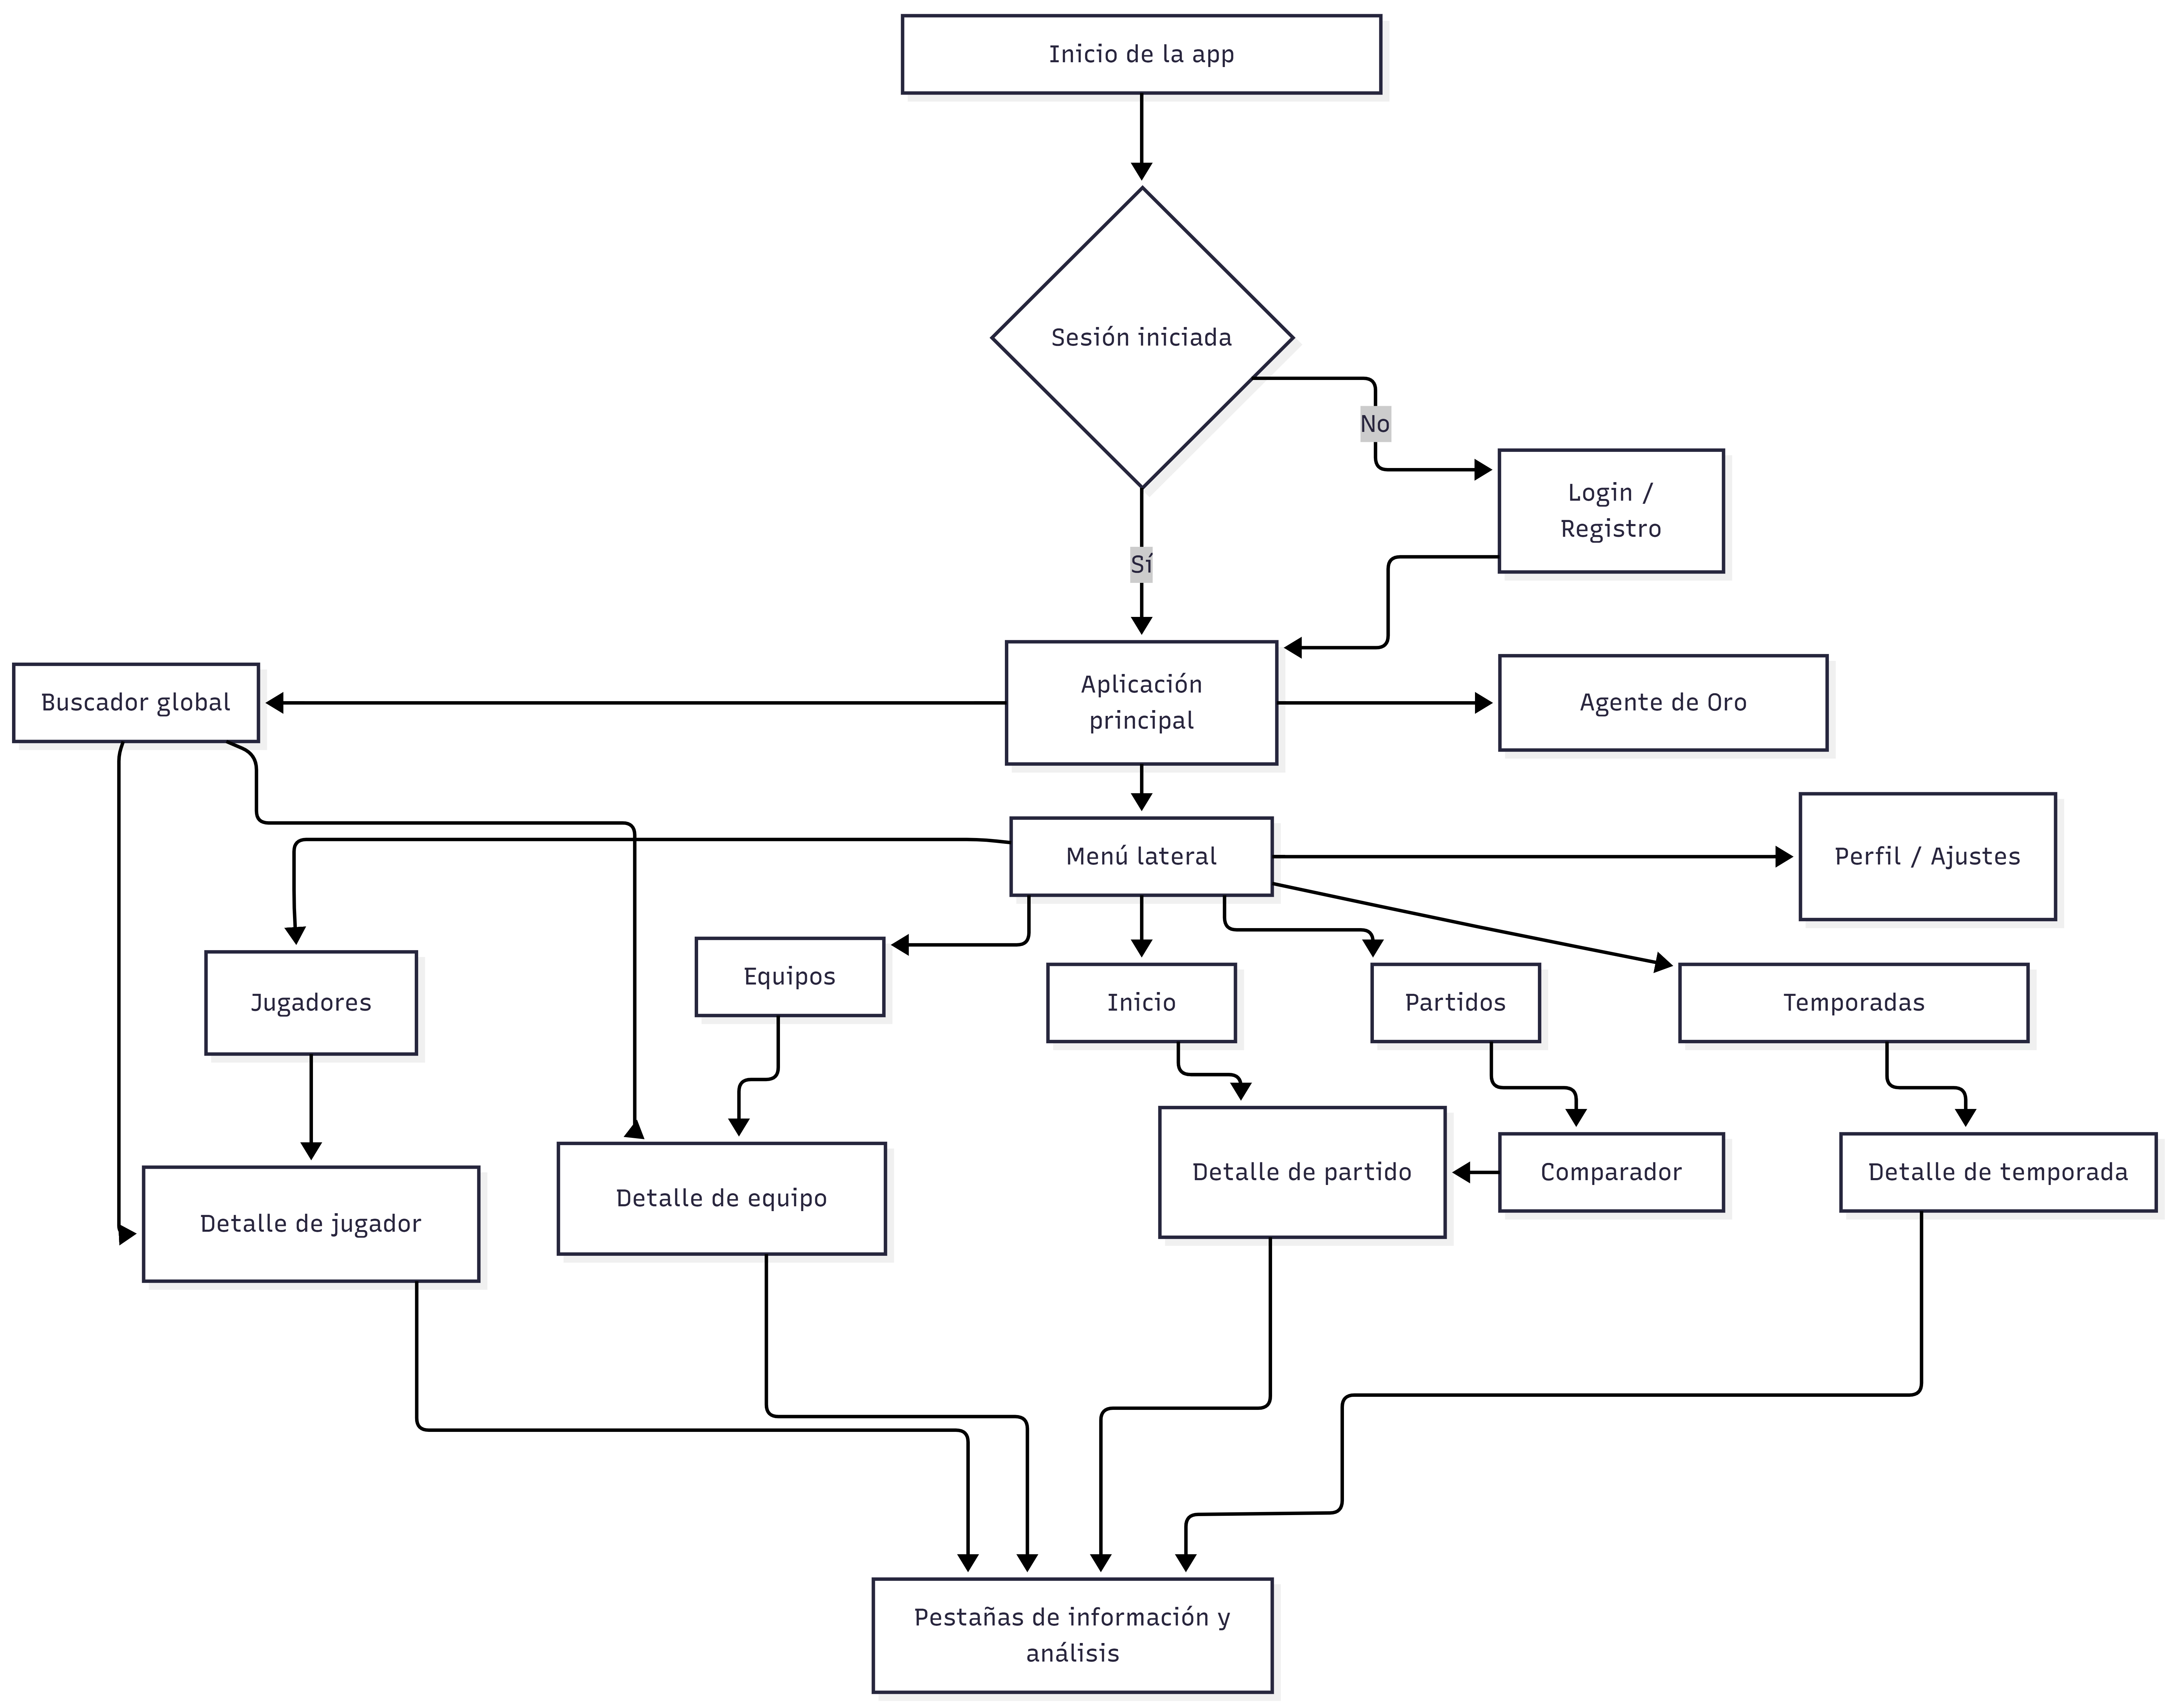
\includegraphics[width=1\linewidth]{figures/navegación.png}
    \caption{Diagrama de navegación.}
    \label{fig:navegacion}
\end{figure}